% last update november 2019
\documentclass{esannV2}
\usepackage{graphicx}
\usepackage[utf8]{inputenc}
\usepackage{amssymb,amsmath,array}
\usepackage{hyperref}
\usepackage{booktabs}
\usepackage{tikz}
\usepackage[english]{babel}
\usetikzlibrary{positioning,shapes.geometric,arrows.meta,calc}
\usepackage{xcolor}

% ==== New commands =========================
\newcommand{\rgg}[2]{{\textcolor{blue}{#2}}}

%=============================================
%***********************************************************************
% !!!! IMPORTANT NOTICE ON TEXT MARGINS !!!!!
%***********************************************************************
%
% Please avoid using DVI2PDF or PS2PDF converters: some undesired
% shifting/scaling may occur when using these programs
% It is strongly recommended to use the DVIPS converters, and to submit
% PS file. You may submit a PDF file if and only if you use ADOBE ACROBAT
% to convert your PS file to PDF.
%
% Check that you have set the paper size to A4 (and NOT to letter) in your
% dvi2ps converter, in Adobe Acrobat if you use it, and in any printer driver
% that you could use.  You also have to disable the 'scale to fit paper' option
% of your printer driver.
%
% In any case, please check carefully that the final size of the top and
% bottom margins is 5.2 cm and of the left and right margins is 4.4 cm.
% It is your responsibility to verify this important requirement.  If these margin requirements and not fulfilled at the end of your file generation process, please use the following commands to correct them.  Otherwise, please do not modify these commands.
%
\voffset 0 cm \hoffset 0 cm \addtolength{\textwidth}{0cm}
\addtolength{\textheight}{0cm}\addtolength{\leftmargin}{0cm}

%***********************************************************************
% !!!! USE OF THE esannV2 LaTeX STYLE FILE !!!!!
%***********************************************************************
%
% Some commands are inserted in the following .tex example file.  Therefore to
% set up your ESANN submission, please use this file and modify it to insert
% your text, rather than staring from a blank .tex file.  In this way, you will
% have the commands inserted in the right place.

\begin{document}
%style file for ESANN manuscripts
\title{See Without Decoding: Motion-Vector-Based Tracking in Compressed Video}

%***********************************************************************
% AUTHORS INFORMATION AREA
%***********************************************************************
\author{Duch\'e Axel$^{1,2}$, Gasso Gilles$^2$ and Chatelain Cl\'ement $^2$
%
% Optional short acknowledgment: remove next line if non-needed
\thanks{This work was supported by the ANRT under a CIFRE contract with Actemium Paris Transport.}
%
% DO NOT MODIFY THE FOLLOWING '\vspace' ARGUMENT
\vspace{.3cm}\\
%
% Addresses and institutions (remove "1- " in case of a single institution)
1- Actemium Paris Transport, %\\
%24 Bd de Pesaro, 92000 
Nanterre - France\\
%
% Remove the next three lines in case of a single institution
2- INSA Rouen, LITIS UR 4108, Saint-Étienne-du-Rouvray - France
}
%***********************************************************************
% END OF AUTHORS INFORMATION AREA
%***********************************************************************

\maketitle

\begin{abstract}
We propose a lightweight \textbf{compressed-domain tracking model} that operates directly on video streams, %\rgg{eliminating full RGB decompression}
without requiring full RGB video decoding. Using motion vectors and transform coefficients from compressed data, our deep model propagates object bounding boxes across frames, 
achieving a computational speed-up of order up to $7\times$ with only a slight 4\% mAP@0.5 drop vs RGB baseline on MOTS15/17/20. These results highlight codec-domain motion modeling efficiency for real-time analytics in large monitoring systems.%reducing computational cost by up to $7\times$ with only 4\% mAP@0.5 drop vs RGB baseline on MOTS15/17/20. These results highlight codec-domain motion modeling efficiency for real-time analytics in large monitoring systems.
\end{abstract}

\section{Introduction}
\label{sec:intro}

Modern cities operate extensive camera networks across transportation hubs, public areas, and sensitive zones. These systems must deliver reliable, continuous analytics---including motion detection, intrusion monitoring, and behavior analysis---under strict constraints on computation, storage, and energy consumption across thousands of concurrent video streams. Conventional image-domain preprocessing~\cite{PIDS_Survey_2022} (e.g., background subtraction or frame differencing) offers low-cost activity filtering but remains fragile under illumination changes, vibrations and clutter.
%
Deep learning--based vision models have substantially improved robustness and precision while maintaining a good balance between speed and accuracy, as seen in recent architectures such as RT-DETR~\cite{detrs_beat_yolos_2024} and the latest YOLO versions~\cite{khanam2024yolov11overviewkeyarchitectural}. However, most %vision pipelines 
methods still rely on fully decoded RGB frames, which are computationally heavy and memory-intensive to process. Performing real-time inference on high-resolution RGB data requires powerful GPUs or specialized hardware, making large-scale deployment difficult and energy-intensive. This dependency on heavy RGB processing represents a fundamental scalability barrier for camera networks.

%We address 
The paper addresses this limitation by starting from %a simple hypothesis
the following assumption: compressed video streams already carry most of the spatial–temporal information required for tracking. In particular, motion vectors and transform coefficients estimated by the codec can %be reused 
act as meaningful motion and appearance cues without explicit RGB reconstruction. Building on this, %assumption, we propose 
the paper proposes a lightweight hybrid architecture that performs a single detection on an initial decoded RGB frame, followed by tracking and refinement of bounding boxes directly from codec-domain features. By leveraging information already available in the stream, the %system 
method avoids redundant pixel-level computation while maintaining competitive accuracy, supporting scalable and energy-efficient analytics across large camera infrastructures.

%Hereafter, we briefly review prior research on compressed-domain video understanding and how existing strategies balance efficiency and accuracy under similar constraints.
Hereafter, we first explain the compressed video representation that enables our approach, then review prior work on compressed-domain video understanding and how these methods balance efficiency and accuracy under similar constraints.


\section{Compressed Video and Related Work}
\label{sec:sota}

\subsection{Compressed Video Representation}
\label{subsec:compressed_representation}

Standard video codecs (e.g., MPEG-4, H.264) organize streams into \emph{Groups of Pictures} (GOPs) $\mathcal{G}^g=\{f_0^g, f_1^g, \ldots, f_N^g\}$, where $f_0^g$ is a fully encoded RGB image and temporal frames $f_n^g$ ($n>0$) are encoded via block motion estimation (Fig.~\ref{fig:motion_estimation}).

\begin{figure}[h!]
\centering
\includegraphics[width=0.95\linewidth]{figs/motion_block_estimation}
\caption{Block motion estimation in MPEG-4: the encoder searches for matching blocks between consecutive frames, computing motion vectors $MV_n^g$ and residuals $\Delta Y_n^g$ (pixel subtraction). The search zone shows candidate blocks explored during estimation.}
\label{fig:motion_estimation}
\vspace{-0.4em}
\end{figure}

Each P-frame contains two key components:
\[
f_n^g = \{MV_n^g, \Delta Y_n^g\},
\qquad
f_0^g = \{\mathcal{DCT}(Y_0^g)\}.
\]
Motion vectors $MV_n^g$ capture block-wise displacement by searching for matching blocks within a search zone, while residuals $\Delta Y_n^g$ encode appearance differences via pixel subtraction.
Since MPEG-4 applies Discrete Cosine Transform (DCT) to compress residuals, we directly work with DCT coefficients that compactly represent texture, edges, and appearance changes in the frequency domain.
To reduce computational cost, we operate exclusively on the luminance (Y) channel---equivalent to a grayscale image---cutting data volume by $\sim$3$\times$ while preserving spatial-temporal structure for tracking.


\paragraph{Efficiency.}
These codec features are already computed during encoding, making them extractable from the bitstream at minimal cost---a key advantage for large-scale video analytics.
\textbf{Motion vectors are dramatically more compact than RGB images} (384$\times$ smaller), providing efficient motion cues at negligible memory cost.
DCT residuals, while having the same spatial resolution as grayscale images (80$\times$80 for 8$\times$8 blocks), can be further compressed by the energy-compaction properties of the DCT transform---similar to JPEG compression---concentrating information in low-frequency coefficients and enabling potential data reduction as exploited in standard compression pipelines.

\subsection{Related Work and Positioning}
Codec-domain features already computed during video encoding provide compact motion and appearance cues at minimal cost.  
However, existing methods differ in how much of the original RGB data they reconstruct before inference.  
They can be broadly categorized into three decoding regimes: \emph{full}, \emph{partial}, and \emph{none}.  
Full-decoding approaches restore complete RGB frames for analysis, achieving strong accuracy but at high computational expense.  
Partial-decoding methods limit reconstruction to selected regions or frames, reducing cost while retaining spatial detail.  
Finally, no-decoding models work directly on compressed-domain data such as motion vectors or transform coefficients, maximizing efficiency for large-scale video analytics.




\paragraph{Full decoding.}
Conventional approaches fully reconstruct RGB frames before analysis.  
They rely on convolutional or transformer-based deep models to detect and track objects in the pixel domain, achieving high accuracy but at a substantial computational cost.  
Methods such as MV-YOLO~\cite{mv_yolo_motion_vector_2018}, originally designed for city surveillance, and later RGB--motion fusion variants like MV-Soccer~\cite{majeed2024mvsoccer} and ReST~\cite{majeed2025rest}, for sports tracking, all exploit codec motion vectors alongside RGB cues to enhance temporal consistency.  
Although this design effectively leverages motion information, it still depends on full-resolution RGB decoding and deep feature extractors, resulting in architectures that are accurate but computationally demanding and difficult to scale for large, real-time video analytics.

\paragraph{Partial decoding.}
To reduce overhead, a few methods leverage motion and residual information computed by the codec while still decoding parts of the frame.  Frame-group aggregation methods~\cite{wang2019fastobjectdetectioncompressed,Wang_2021} process one GOP at a time, using the initial decoded RGB I-frame together with decompressed residuals and motion vectors to predict objects across subsequent frames.  
While this design effectively exploits temporal redundancy and achieves strong accuracy, many of its internal operations—such as feature resizing and residual decompression—are not computationally optimal, limiting the overall speed and efficiency.  
Other hybrid designs~\cite{Fast_Object_Detection_in_High-Resolution_Videos_2023} decode small regions or key patches while combining them with motion cues from the bitstream.  
However, because video data are sequentially encoded, even partial decoding typically requires decoding earlier related patches, which limits the achievable efficiency.


\paragraph{No-decoding methods.}
Recent studies~\cite{chen2021fasthevc,elkhoury2021deep,dct_detection_2019,dct_luminance_2021} explore learning directly from compressed-domain data without reconstructing RGB pixels.  
Among them, \cite{chen2021fasthevc} and \cite{dct_detection_2019} focus on object detection in still images compressed with HEVC-Intra and JPEG respectively, showing that partitioning depths, prediction modes, and transform coefficients preserve sufficient spatial structure for localization.  
However, these image-oriented designs cannot be directly extended to video, where temporal dependencies and motion cues play a critical role beyond static spatial transformations.  
In contrast, video-oriented methods~\cite{elkhoury2021deep,dct_luminance_2021} rely exclusively on motion vectors and residuals extracted from compressed streams.  
While efficient, these architectures struggle to handle static or slow-moving objects, since such regions generate little or no motion information in the bitstream, leading to incomplete scene representation.  
Nevertheless, this last class of models remains the most suitable for minimizing computational cost and energy consumption, making it a promising direction for scalable, power-efficient video analytics.
\paragraph{Our contribution} Building on the latter idea, we propose a lightweight \emph{tracking model} that performs a single detection on an initial decoded frame and then updates bounding boxes using only motion vectors and \rgg{transform coefficients}{frequency domain features} from the compressed stream.  
Unlike full or partial decoding-based approaches, our formulation %removes the need for 
avoids repeated RGB reconstruction and heavy temporal aggregation, operating entirely on data already present in the bitstream.  
This design retains essential motion and appearance cues while drastically reducing computational burden, making it suitable for real-time, large-scale video analytics.

\section{See Without Decoding using BAFE}
\label{sec:architecture}

Our approach initializes bounding boxes via RGB-based detection on I-frame $f_0^g$, then propagates them across P-frames using only codec features (motion vectors, DCT coefficients) extracted directly from the bitstream without full RGB decoding. 

\textbf{BAFE (Box-Aligned Feature Extraction).} Unlike global pooling approaches that process entire frames, our architecture extracts features \emph{spatially aligned} with each bounding box. For each box $b_n^i$ at frame $f_n^g$, we extract fixed-size grid features from the bounding box region in motion vectors $MV_n^g$ and DCT coefficients $\Delta Y_n^g$. For videos of size $960 \times 960$ pixels with mean bounding box resolution of $240 \times 240$, we use a $15 \times 15$ grid for motion vectors (matching the spatial resolution of 16-pixel macroblocks). For DCT coefficients, where each $8 \times 8$ pixel block yields 64 frequency channels, we employ a $30 \times 30$ grid to capture finer-grained appearance details. This box-aligned extraction focuses computation on object regions while ignoring background, enabling lightweight processing ($\sim$230K params) compared to full-frame architectures. Each extracted region is processed through shallow convolutional layers (2 Conv blocks, 64 channels) to produce compact $128$-dimensional feature embeddings.

\textbf{BiLSTM Temporal Propagation.} To model temporal dependencies across P-frames, we employ a bidirectional LSTM that takes as input the concatenation of: (1) box-aligned motion vector features from $MV_n^g$, (2) box-aligned DCT coefficient features from $\Delta Y_n^g$, and (3) encoded bounding box geometry (position/size of $b_{n-1}^i$). The BiLSTM hidden state captures motion patterns over time, enabling the model to predict refined bounding box updates $\Delta b_n^i = (\Delta x, \Delta y, \Delta w, \Delta h)$ relative to the previous frame. This temporal modeling is crucial for handling occlusions, camera motion, and non-linear trajectories that simple motion vector averaging cannot capture.
\begin{figure}[h!]
\centering
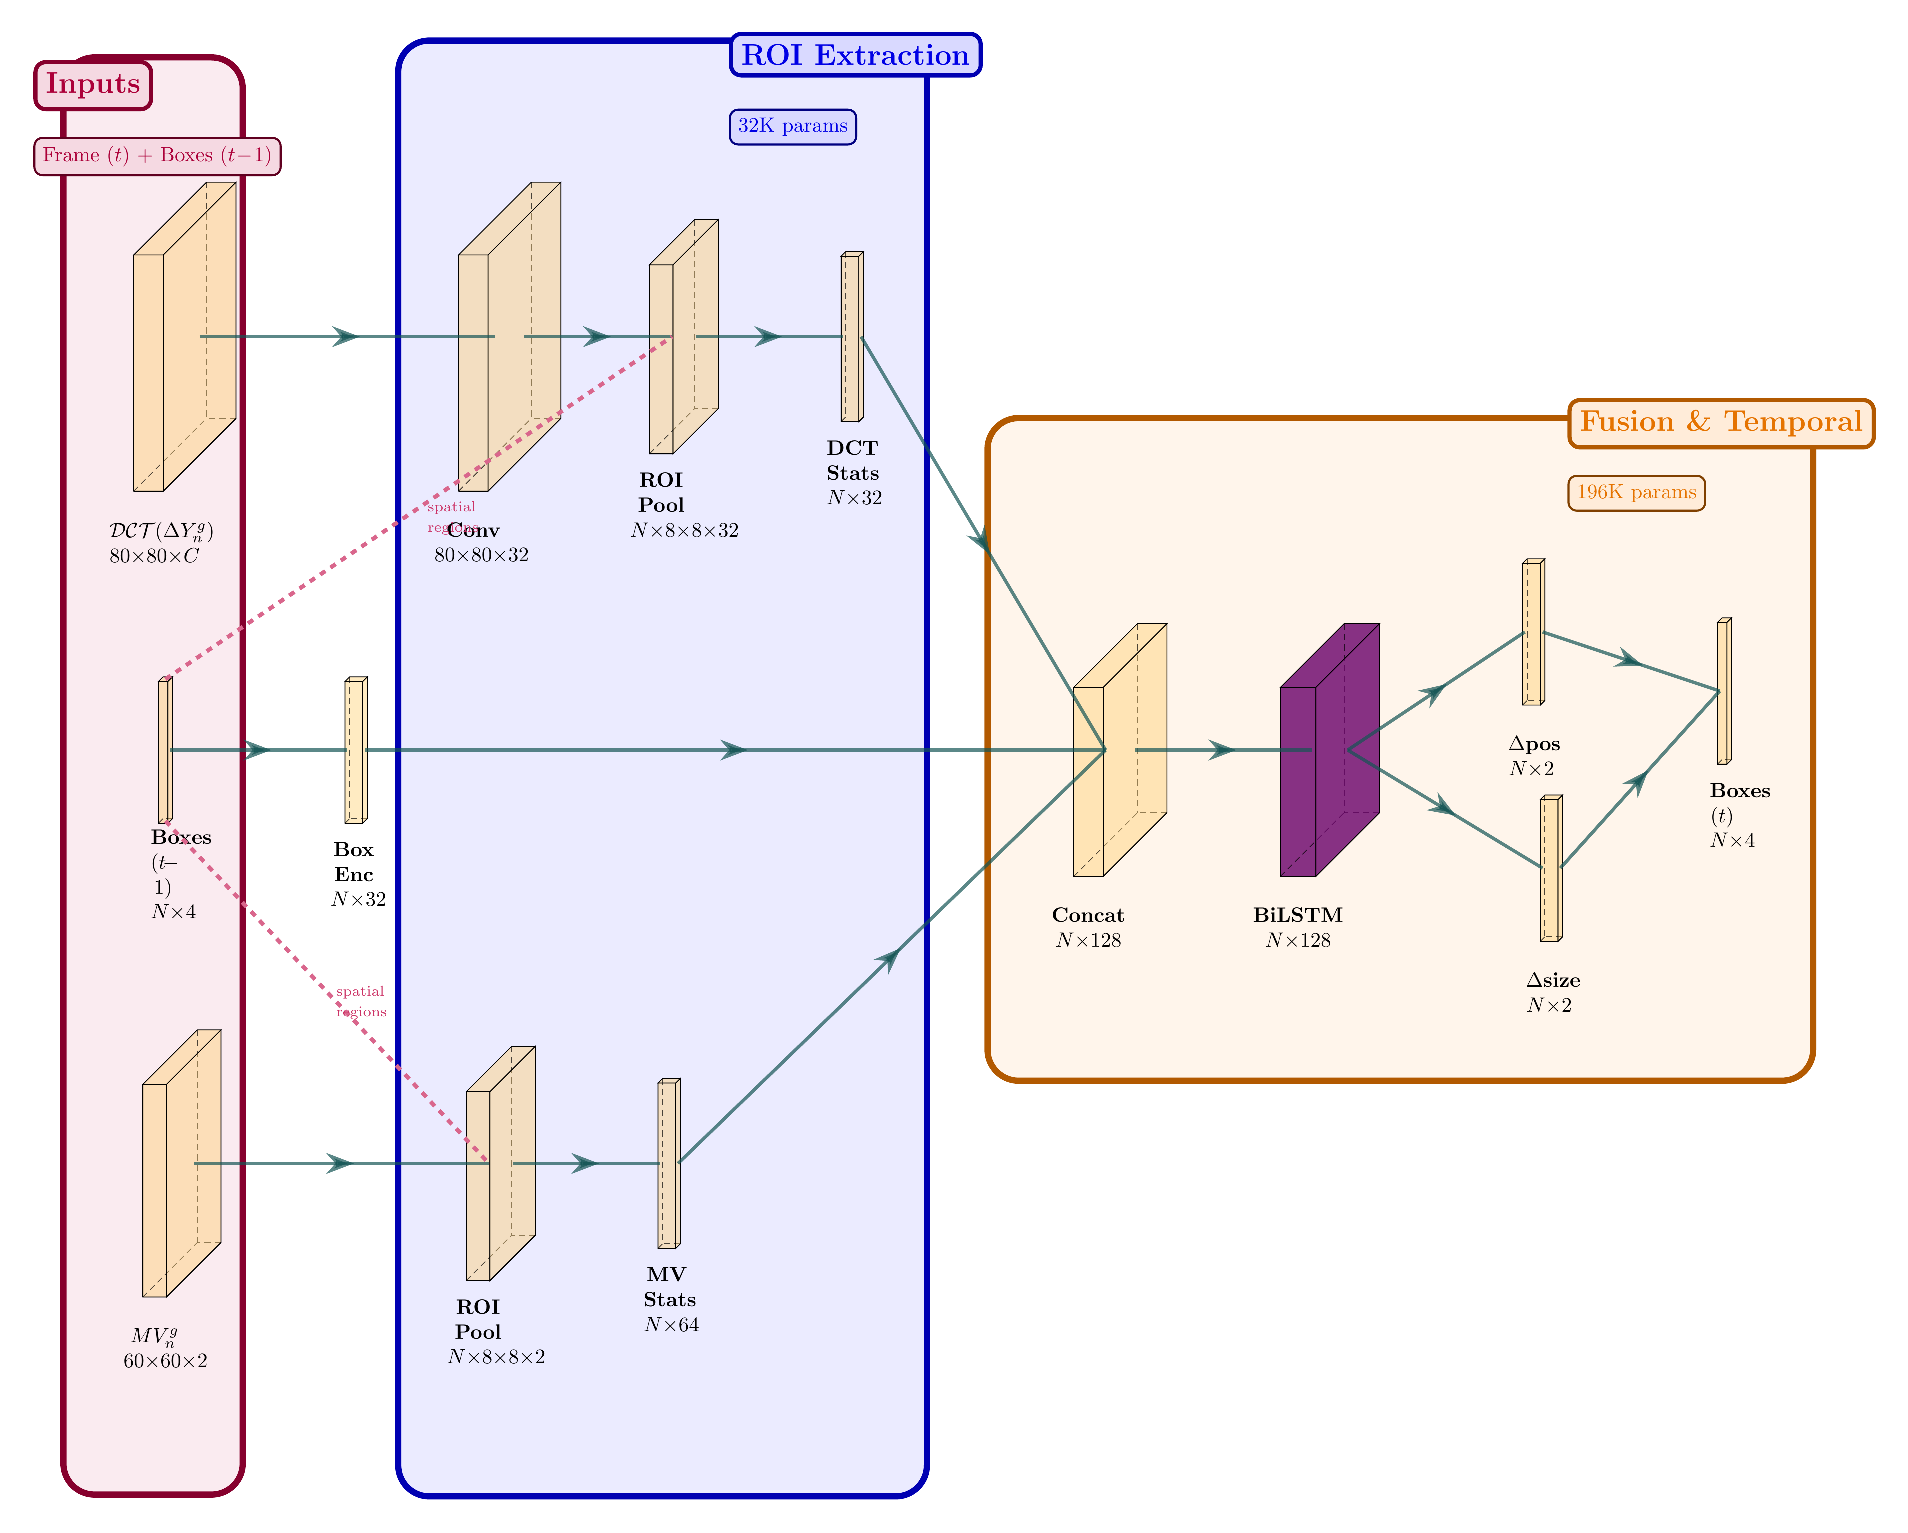
\includegraphics[width=1.2\linewidth]{figs/roi_architecture}
\caption{BAFE architecture: box-aligned MV/DCT features fused with box encodings, BiLSTM for temporal modeling.}
\label{fig:roi_architecture}
\end{figure}

\textbf{Addressing SOTA Limitations.} Our hybrid approach resolves three key problems in compressed-domain tracking: (1) \emph{vs. no-decoding methods}~\cite{elkhoury2021deep,dct_luminance_2021}: by using RGB-based detection on $f_0^g$, we obtain high-quality initial boxes that enable tracking of static or slow-moving objects (which purely motion-based methods miss); (2) \emph{vs. full-decoding methods}~\cite{mv_yolo_motion_vector_2018,majeed2024mvsoccer}: after the initial I-frame, we never reconstruct RGB images, avoiding computational overhead of repeated decoding; (3) \emph{vs. partial-decoding methods}~\cite{wang2019fastobjectdetectioncompressed,Wang_2021}: we operate directly on bitstream features without selective decoding, eliminating synchronization overhead and codec-specific optimizations. The initial bounding boxes serve as strong priors that transform the challenging detection problem into a simpler tracking problem, where codec features suffice for propagation.

\section{Experimental Results}
\label{sec:results}

We evaluate on MOT15/17/20 static cameras with baselines: \textbf{RT-DETR} (RGB-based detection per frame) and \textbf{Mean MV} (average motion vector per box). The MOT datasets focus on pedestrian tracking from surveillance camera recordings. All model variants are trained using DETR-style bounding box regression losses (focal loss for center prediction, L1 and GIoU for box geometry) on 200 GOPs of size 6. Since the tracking task involves a single pedestrian class, no classification head or cross-entropy loss is used---the model directly predicts box refinements $\Delta b_n^i$ from codec features. Table~\ref{tab:results_compact} presents GOP-6 performance (1I+5P), where our best BAFE model (MV+DCT) achieves \textbf{0.8962 mAP} on MOT17, outperforming Mean MV by \textbf{+2.86\%} while staying within \textbf{2.25\%} of the RGB baseline. On \textbf{MOT15}, the model gains \textbf{+20.79\%} over Mean MV by learning temporal patterns for fast-moving pedestrians. The MV-only variant maintains strong performance (\textbf{0.8756 mAP} on MOT17), demonstrating that motion cues alone suffice for accurate tracking when combined with learned temporal modeling.

\begin{table}[h!]
\centering
\setlength{\tabcolsep}{3pt}
\renewcommand{\arraystretch}{1.05}
\caption{BAFE model performance on static cameras (GOP-6, mAP@0.5).}
\label{tab:results_compact}
\begin{tabular}{|l|c|c|c|c|}
\hline
\textbf{Metric} & \textbf{MOT17} & \textbf{MOT15} & \textbf{MOT20} \\
\hline
\textbf{Baseline RGB (RT-DETR)} & \textbf{0.9187} & \textbf{0.8234} & \textbf{0.8153} \\
\textbf{Mean MV} & 0.8676 & 0.5879 & 0.6590 \\
\textbf{BAFE Model (MV) } & \textbf{0.8756} &  \textbf{0.7851}  & \textbf{0.7990} \\
\hline
\textbf{BAFE Model (DCT) } & 0.8543 &  0.7564  & 0.7843 \\
\hline
\textbf{BAFE Model (MV+DCT) } & \textbf{0.8962} &  \textbf{0.7958}  & \textbf{0.8020} \\
\hline
\textbf{Our Model (Best) vs Mean MV} & \textbf{+0.0286} & \textbf{+0.2079} & \textbf{+0.1430} \\
\hline
\textbf{Our Model (Best) vs RT-DETR} & -0.0225 & -0.0276 & -0.0133 \\
\hline
\textbf{Our Model (MV) vs RT-DETR} & -0.0431 & -0.0383 & -0.0163 \\
\hline
\end{tabular}
\vspace{-0.4em}
\end{table}

\paragraph{Deployment Scalability.}
Table~\ref{tab:speed_gop} shows deployment capacity on 16GB GPU for GOP-6 (1I+5P). Despite its compact 160K parameters, our MV-only variant processes \textbf{71 concurrent streams} vs. \textbf{13 streams} for RT-DETR (32M params), achieving \textbf{5.5$\times$ throughput} with 200$\times$ fewer parameters. The lightweight Mean MV baseline (no learned parameters) handles 85 streams but sacrifices 20\% mAP compared to our learned model. MV+DCT and DCT variants (230K and 202K params) support 21-23 streams while maintaining competitive accuracy, demonstrating flexible accuracy-throughput trade-offs for different deployment scenarios.

\begin{table}[h!]
\centering
\setlength{\tabcolsep}{4pt}
\renewcommand{\arraystretch}{1.05}
\caption{Deployment capacity on 16GB GPU (30 FPS streams) for GOP-6 (1I+5P).}
\label{tab:speed_gop}
\begin{tabular}{lcc}
\toprule
\textbf{Variant} & \textbf{Concurrent Streams} & \textbf{Parameters} \\
\midrule
RT-DETR (RGB) & 13 & 32M \\
Mean MV & 85 & 0 \\
BAFE Model (MV) & \textbf{71} & \textbf{160K} \\
BAFE Model (MV+DCT) & 21 & 230K \\
BAFE Model (DCT) & 23 & 202K \\
\bottomrule
\end{tabular}
\vspace{-0.5em}
\end{table}

\paragraph{Discussion.}
Our learned BAFE models significantly outperform the naive Mean MV baseline (+2.9\% to +20.8\% across datasets), demonstrating that temporal modeling via BiLSTM effectively captures motion patterns beyond simple vector averaging. Notably, the MV-only variant achieves competitive accuracy (0.8756 mAP on MOT17) with only a 2.1\% gap relative to MV+DCT (0.8962 mAP), suggesting motion vectors alone carry sufficient information for tracking when properly exploited through learned features. This validates the potential of codec-domain motion as a primary cue for video analytics.

Speed analysis reveals that throughput differences stem primarily from input data size rather than model complexity: MV-only (71 streams, 160K params) outperforms MV+DCT (21 streams, 230K params) by 3.4$\times$ despite similar architectures, highlighting the compactness advantage of motion vectors (384$\times$ smaller than images). Comparing our variants (21-71 streams, 160-230K params) against RT-DETR (13 streams, 32M params) confirms that efficient feature extraction at codec level---not just model size---drives scalability.

Future work could explore multi-scale bounding box grids inspired by YOLO-style feature pyramids to better handle scale variations, and selective DCT frequency exploitation (leveraging energy-compaction properties) to improve appearance modeling without sacrificing the current throughput advantages. Additionally, incorporating explicit object identity tracking (e.g., learnable ID embeddings) could further improve temporal consistency, as the current model operates purely on geometric and codec features without identity-aware associations across frames.


% ****************************************************************************
% BIBLIOGRAPHY AREA
% ****************************************************************************

\begin{footnotesize}

% IF YOU DO NOT USE BIBTEX, USE THE FOLLOWING SAMPLE SCHEME FOR THE REFERENCES
% ----------------------------------------------------------------------------
\begin{thebibliography}{99}

% --- Core real-time detection & transformers ---

\bibitem{PIDS_Survey_2022}
D. Lohani, C. Crispim-Junior, Q. Barth\'elemy, S. Bertrand, L. Robinault and L. Tougne Rodet,
Perimeter Intrusion Detection by Video Surveillance: A Survey, MDPI, 2022

\bibitem{detrs_beat_yolos_2024}
Y. Zhao, W. Lv, S. Xu, J. Wei, G. Wang, Q. Dang, Y. Liu, and J. Chen,
``DETRs Beat YOLOs on Real-Time Object Detection, CVPR, 2024


\bibitem{khanam2024yolov11overviewkeyarchitectural}
R. Khanam and M. Hussain,
YOLOv11: An Overview of the Key Architectural Enhancements, ARXiV, 2024

\bibitem{mv_yolo_motion_vector_2018}
S. R. Alvar and I. V. Baji\'c,
MV-YOLO: Motion Vector-aided Tracking by Semantic Object Detection, IEEE International Workshop on Multimedia Signal Processing,  2018.

\bibitem{wang2019fastobjectdetectioncompressed}
S.~Wang, H.~Lu, and Z.~Deng, ``Fast Object Detection in Compressed Video, ICCV, 2018

\bibitem{Wang_2021}
X. Wang, Z. Huang, B. Liao, L. Huang, Y. Gong and C. Huang,
Real-time and accurate object detection in compressed video by long short-term feature aggregation, CVIU, 2021.

\bibitem{Fast_Object_Detection_in_High-Resolution_Videos_2023}
R. Tran, A. Kanaujia and V. Parameswaran,
Fast Object Detection in High-Resolution Videos, ICCVW, October 2023.

\bibitem{dct_detection_2019}
B. Deguerre, C. Chatelain and G. Gasso,
Fast object detection in compressed JPEG images, ITSC , 2019.

\bibitem{dct_luminance_2021}
B. Deguerre, C. Chatelain and G. Gasso,
Object Detection in the DCT Domain: is Luminance the Solution, ICPR 2020

\bibitem{MOTS15}
L. Leal-Taix\'{e}, A. Milan, I. Reid, S. Roth, and K. Schindler,
``MOTChallenge 2015: Towards a Benchmark for Multi-Target Tracking

\bibitem{MOTS17}
A. Milan, L. Leal-Taix\'{e}, I. Reid, S. Roth, and K. Schindler,
``MOT16: A Benchmark for Multi-Object Tracking

\bibitem{MOTS20}
P. Dendorfer, H. Rezatofighi, A. Milan, J. Shi, D. Cremers, I. Reid, S. Roth, K. Schindler, and L. Leal-Taix\'{e},
``MOT20: A Benchmark for Multi-Object Tracking in Crowded Scenes

\bibitem{majeed2024mvsoccer}
F.~Majeed, N.~U. Gilal, K.~Al-Thelaya, Y.~Yang, M.~Agus, and J.~Schneider,
``MV-Soccer: Motion-Vector Augmented Instance Segmentation for Soccer Player Tracking,''
in \emph{Proceedings of the IEEE/CVF Conference on Computer Vision and Pattern Recognition Workshops (CVPRW)}, 
June 2024, pp.~3245--3255, doi:10.1109/CVPRW63382.2024.00330.

\bibitem{majeed2025rest}
F.~Majeed, K.~A.~L. Al-Thelaya, N.~U. Gilal, K.~Swart-Arries, M.~Agus, and J.~Schneider,
``ReST: High-Precision Soccer Player Tracking via Motion Vector Segmentation,''
in \emph{Proceedings of the 20th International Joint Conference on Computer Vision, Imaging and Computer Graphics Theory and Applications (VISIGRAPP)}, 
vol.~2, 2025, pp.~138--149, doi:10.5220/0013168000003912.

\bibitem{chen2021fasthevc}
L.~Chen, Y.~Li, C.~Hou, and Z.~Gao,
``Fast Object Detection in HEVC Intra Compressed Domain,''
in \emph{Proceedings of the 29th European Signal Processing Conference (EUSIPCO)}, 
Dublin, Ireland, Aug.~2021, pp.~756--760.

\bibitem{elkhoury2021deep}
K.~El Khoury, J.~Samelson, and B.~Macq,
``Deep Learning-Based Object Tracking via Compressed Domain Residual Frames,''
\emph{Frontiers in Signal Processing}, vol.~1, Nov. 2021, article 765006. doi:10.3389/frsip.2021.765006.

\bibitem{he2017mask}
K.~He, G.~Gkioxari, P.~Doll\'ar, and R.~Girshick,
``Mask R-CNN,''
in \emph{Proceedings of the IEEE International Conference on Computer Vision (ICCV)}, 
Oct.~2017, pp.~2961--2969.

\end{thebibliography}


% ----------------------------------------------------------------------------

% IF YOU USE BIBTEX,
% - DELETE THE TEXT BETWEEN THE TWO ABOVE DASHED LINES
% - UNCOMMENT THE NEXT TWO LINES AND REPLACE 'Name_Of_Your_BibFile'

%\bibliographystyle{unsrt}
%\bibliography{Name_Of_Your_BibFile}

\end{footnotesize}

% ****************************************************************************
% END OF BIBLIOGRAPHY AREA
% ****************************************************************************

\end{document}
